\subsection{Geometry vs Volume}

\subsubsection{Geometry and Image Segmentation}
Mario's geometry construction.

\subsubsection{Pipeline: Current State}
Mario's review of the traditional method of image segmentation.

\begin{figure}[h]
 \centering % avoid the use of \begin{center}...\end{center} and use \centering instead (more compact)
 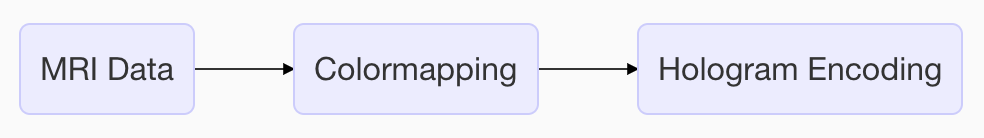
\includegraphics[width=\columnwidth]{pictures/general-model.png}
 \caption{Current State}
 \label{fig:general-model}
\end{figure}

\subsubsection{Volume Observations: Opaque and Translucent Views}
The opaque views create a three simensional form in the viewing space, with defined markings on the brain surface. In figuers 6 through 9, our rendering sample depicts an applied red transmission colour.

% \begin{figure}[ht]
%  \centering % avoid the use of \begin{center}...\end{center} and use \centering instead (more compact)
%  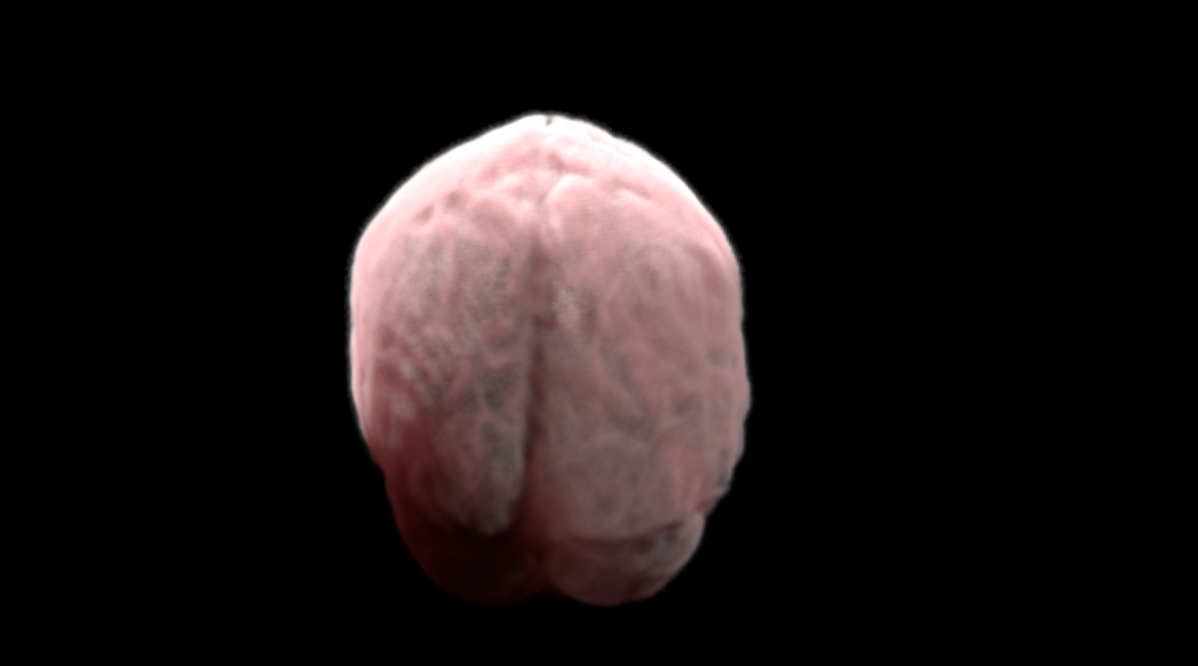
\includegraphics[width=\columnwidth]{pictures/bt-noalphared-front.png}
%  \caption{Opaque MRI Render. Front view.}
%  \label{fig:noalphared-front}
% \end{figure}

\begin{figure}[ht]
 \centering % avoid the use of \begin{center}...\end{center} and use \centering instead (more compact)
 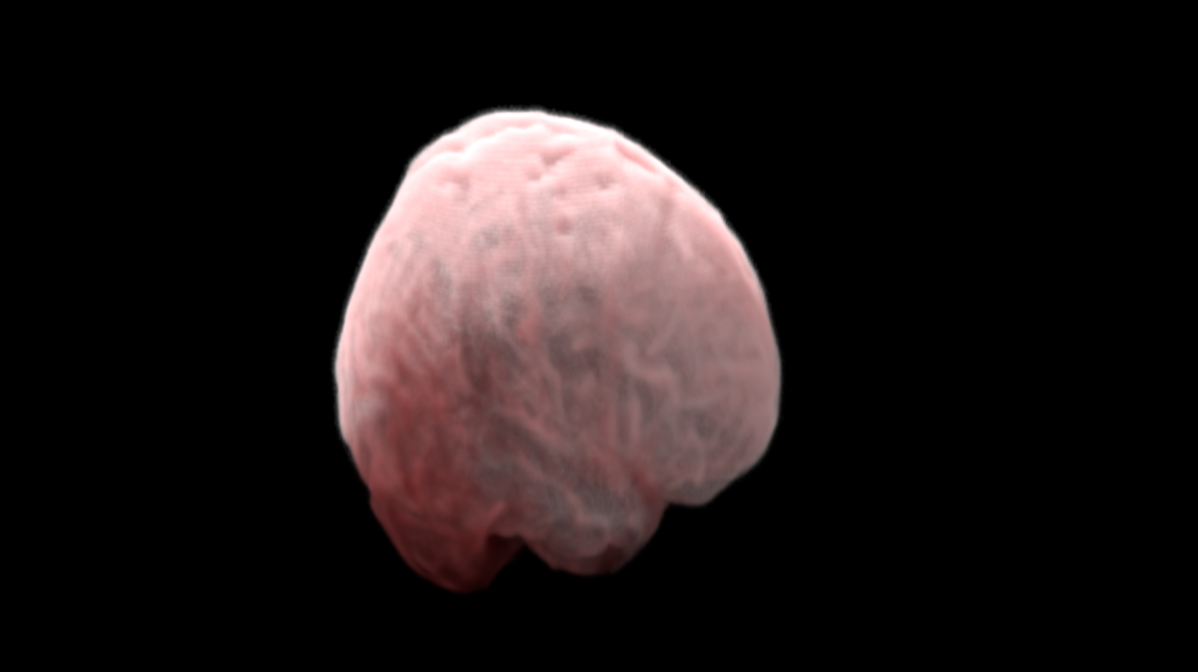
\includegraphics[width=\columnwidth]{pictures/bt-noalphared-lateral.png}
 \caption{Opaque MRI Render. Lateral view.}
 \label{fig:noalphared-lateral}
\end{figure}

\begin{figure}[h]
 \centering % avoid the use of \begin{center}...\end{center} and use \centering instead (more compact)
 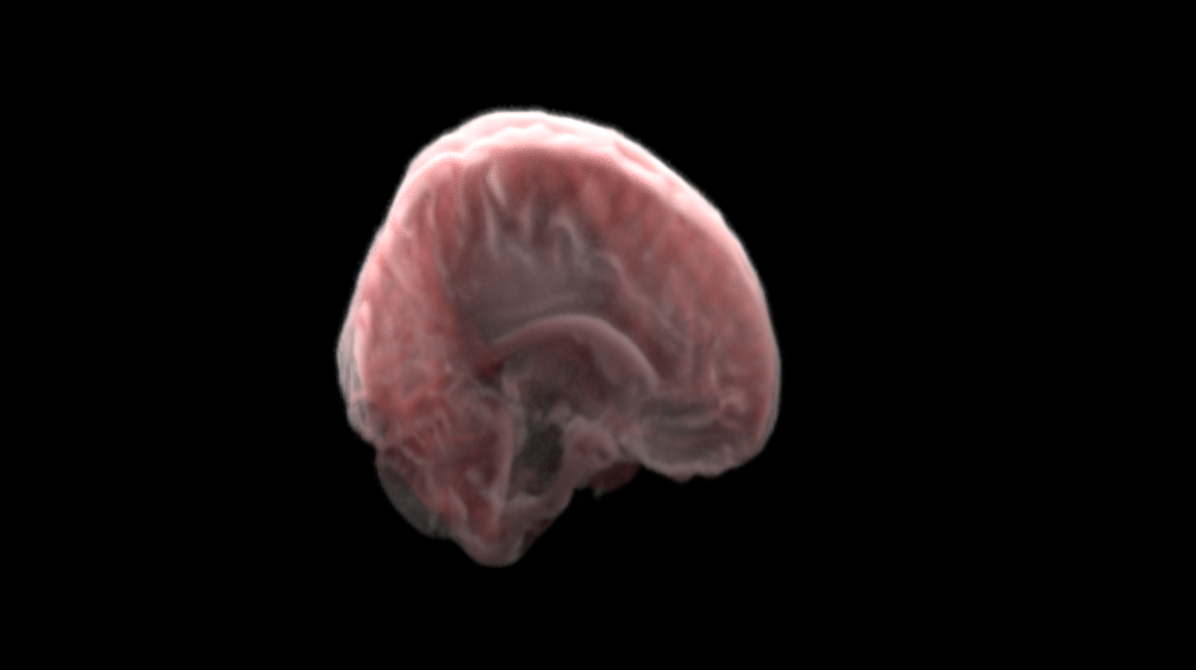
\includegraphics[width=\columnwidth]{pictures/bt-noalphared-lateral-slice.png}
 \caption{Opaque MRI Render. Lateral slice view.}
 \label{fig:noalphared-lateral-slice}
\end{figure}

\begin{figure}[h]
 \centering % avoid the use of \begin{center}...\end{center} and use \centering instead (more compact)
 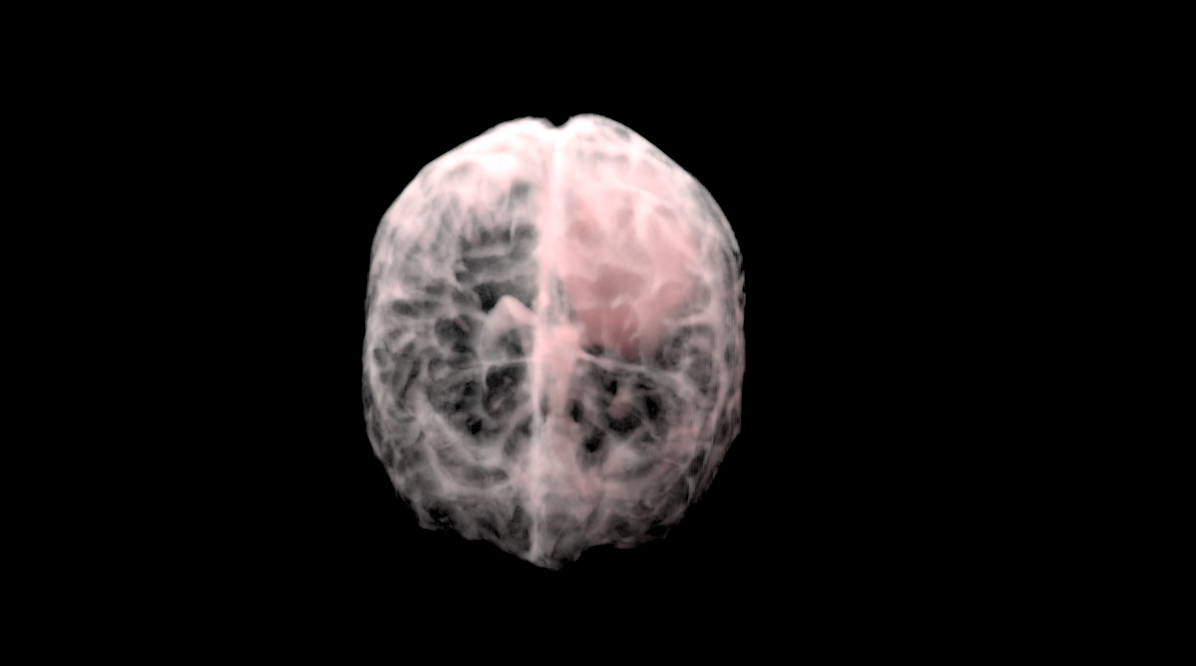
\includegraphics[width=\columnwidth]{pictures/bt-alphared-front.png}
 \caption{Translucent MRI Render. Front view.}
 \label{fig:alphared-front}
\end{figure}

\begin{figure}[h]
 \centering % avoid the use of \begin{center}...\end{center} and use \centering instead (more compact)
 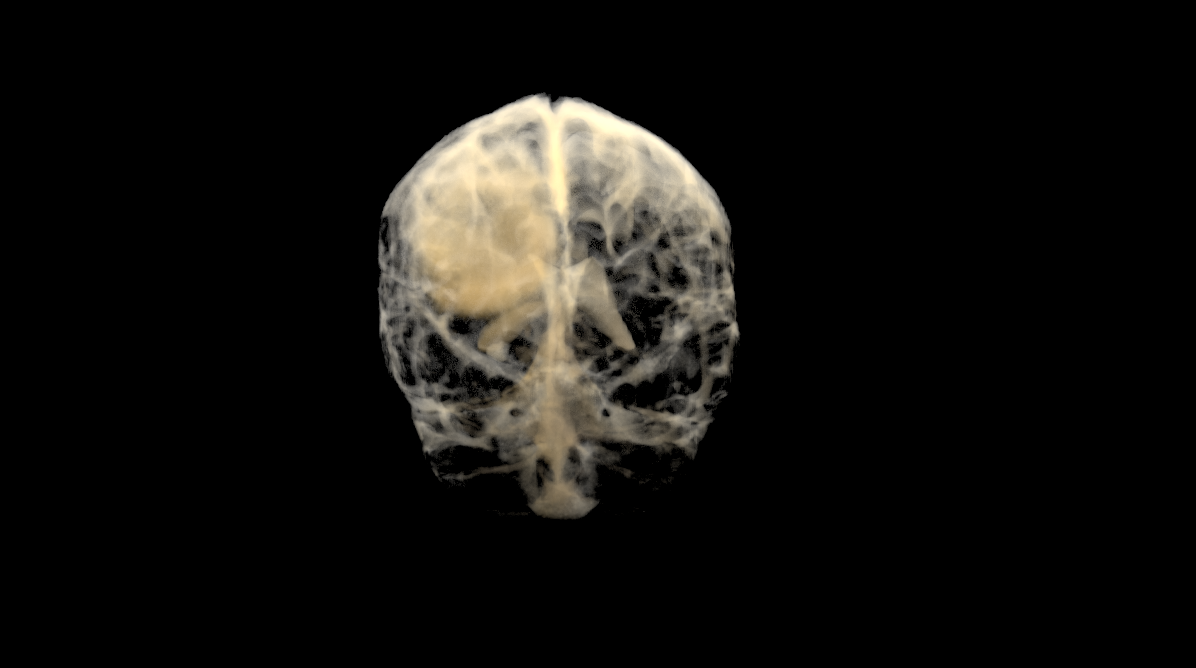
\includegraphics[width=\columnwidth]{pictures/bt-alphalimon-back.png}
 \caption{Translucent MRI Render. Front view.}
 \label{fig:alphared-front}
\end{figure}

Slight opaque regions are revealed from the top down in opaque slices. Translucent slices have a more crystallized look and feel to the image when sliced, however the TC regions are much more prominent.

\subsection{Colour Mapping Methods}
In the CIE 1931 chromaticity diagram, the Y component represents the photopic luminance.  As we know luminance is key to the ability to pinoint detail in segmentation, and the single most important factor in selecting colormaps in this process.  Previous research suggests that luminance is much stronger with colormaps that have two or more interpolation points, and as such has directed our preference towards divergent colormaps and structure colormaps.\\

The search for increased luminance has been the criteria that has steered our research results towards combining forces of an HDR linear workflow, and control of volumetric lighting.  These characteristics of our proposed pipeline are strongly complemented by adding colormaps to the process at either the input stage of MRI data processing or during the volumetric rendering process.  Both methods reveal more insights from the data of the MRI, and create options bringing color snd luminance to the workflows.

\subsection{Pipeline: Proposed Model (Detailed View)}
Our proposal of combined workflows suggests an amalgamation of tasks condensed into three major steps: (1) MRI data preparation, (2) colour mapping, and (3) hologram encoding.  The MRI data preparation involved the extraction of a MRI DICOM or NIFTI medical file of 181 slices for our brain, after which we applied segmentation to isolate the tumour in the image data in traditional DICOM GSDF grayscale.  The colour mapping process was applied to the volume data, and tests show that a divergent and/or structured colormap yield preferred results of highlighting image detail.

\begin{figure}[t]
 \centering % avoid the use of \begin{center}...\end{center} and use \centering instead (more compact)
 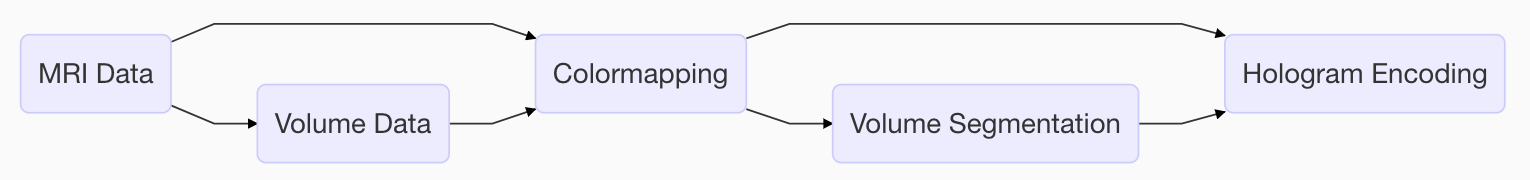
\includegraphics[width=\columnwidth]{pictures/proposed-model.png}
 \caption{Proposed pipeline model}
 \label{fig:proposed-model}
\end{figure}

\subsection{Medical Data Review}
I can't really say anything about this because I do not have any results to speak of.  Meaning we do not have a hologram.  But I was thinking maybe we can create a side by side comparison of the volumetric rendered images with various colour mapping techniques as well as compare them to the geometry based one that was segmented.  Some current ones like gray scale, rainbow and jet, and then we can show our mapping techniques. Then we can talk about the following topics
\begin{itemize}
    \item highlight the advantages of our colour map opposed to others
    \item highlight the importance of geometry vs. volumetric rendering
    \item which one is more true to the medical data (we need Trevor to speak on this)
\end{itemize}
